<<<<<<< HEAD
% GNUPLOT: LaTeX picture with Postscript
\begingroup
  \makeatletter
  \providecommand\color[2][]{%
    \GenericError{(gnuplot) \space\space\space\@spaces}{%
      Package color not loaded in conjunction with
      terminal option `colourtext'%
    }{See the gnuplot documentation for explanation.%
    }{Either use 'blacktext' in gnuplot or load the package
      color.sty in LaTeX.}%
    \renewcommand\color[2][]{}%
  }%
  \providecommand\includegraphics[2][]{%
    \GenericError{(gnuplot) \space\space\space\@spaces}{%
      Package graphicx or graphics not loaded%
    }{See the gnuplot documentation for explanation.%
    }{The gnuplot epslatex terminal needs graphicx.sty or graphics.sty.}%
    \renewcommand\includegraphics[2][]{}%
  }%
  \providecommand\rotatebox[2]{#2}%
  \@ifundefined{ifGPcolor}{%
    \newif\ifGPcolor
    \GPcolorfalse
  }{}%
  \@ifundefined{ifGPblacktext}{%
    \newif\ifGPblacktext
    \GPblacktexttrue
  }{}%
  % define a \g@addto@macro without @ in the name:
  \let\gplgaddtomacro\g@addto@macro
  % define empty templates for all commands taking text:
  \gdef\gplbacktext{}%
  \gdef\gplfronttext{}%
  \makeatother
  \ifGPblacktext
    % no textcolor at all
    \def\colorrgb#1{}%
    \def\colorgray#1{}%
  \else
    % gray or color?
    \ifGPcolor
      \def\colorrgb#1{\color[rgb]{#1}}%
      \def\colorgray#1{\color[gray]{#1}}%
      \expandafter\def\csname LTw\endcsname{\color{white}}%
      \expandafter\def\csname LTb\endcsname{\color{black}}%
      \expandafter\def\csname LTa\endcsname{\color{black}}%
      \expandafter\def\csname LT0\endcsname{\color[rgb]{1,0,0}}%
      \expandafter\def\csname LT1\endcsname{\color[rgb]{0,1,0}}%
      \expandafter\def\csname LT2\endcsname{\color[rgb]{0,0,1}}%
      \expandafter\def\csname LT3\endcsname{\color[rgb]{1,0,1}}%
      \expandafter\def\csname LT4\endcsname{\color[rgb]{0,1,1}}%
      \expandafter\def\csname LT5\endcsname{\color[rgb]{1,1,0}}%
      \expandafter\def\csname LT6\endcsname{\color[rgb]{0,0,0}}%
      \expandafter\def\csname LT7\endcsname{\color[rgb]{1,0.3,0}}%
      \expandafter\def\csname LT8\endcsname{\color[rgb]{0.5,0.5,0.5}}%
    \else
      % gray
      \def\colorrgb#1{\color{black}}%
      \def\colorgray#1{\color[gray]{#1}}%
      \expandafter\def\csname LTw\endcsname{\color{white}}%
      \expandafter\def\csname LTb\endcsname{\color{black}}%
      \expandafter\def\csname LTa\endcsname{\color{black}}%
      \expandafter\def\csname LT0\endcsname{\color{black}}%
      \expandafter\def\csname LT1\endcsname{\color{black}}%
      \expandafter\def\csname LT2\endcsname{\color{black}}%
      \expandafter\def\csname LT3\endcsname{\color{black}}%
      \expandafter\def\csname LT4\endcsname{\color{black}}%
      \expandafter\def\csname LT5\endcsname{\color{black}}%
      \expandafter\def\csname LT6\endcsname{\color{black}}%
      \expandafter\def\csname LT7\endcsname{\color{black}}%
      \expandafter\def\csname LT8\endcsname{\color{black}}%
    \fi
  \fi
    \setlength{\unitlength}{0.0500bp}%
    \ifx\gptboxheight\undefined%
      \newlength{\gptboxheight}%
      \newlength{\gptboxwidth}%
      \newsavebox{\gptboxtext}%
    \fi%
    \setlength{\fboxrule}{0.5pt}%
    \setlength{\fboxsep}{1pt}%
\begin{picture}(4534.00,3400.00)%
    \gplgaddtomacro\gplbacktext{%
      \colorrgb{0.50,0.50,0.50}%
      \put(594,704){\makebox(0,0)[r]{\strut{}$0$}}%
      \colorrgb{0.50,0.50,0.50}%
      \put(594,1111){\makebox(0,0)[r]{\strut{}$20$}}%
      \colorrgb{0.50,0.50,0.50}%
      \put(594,1518){\makebox(0,0)[r]{\strut{}$40$}}%
      \colorrgb{0.50,0.50,0.50}%
      \put(594,1925){\makebox(0,0)[r]{\strut{}$60$}}%
      \colorrgb{0.50,0.50,0.50}%
      \put(594,2332){\makebox(0,0)[r]{\strut{}$80$}}%
      \colorrgb{0.50,0.50,0.50}%
      \put(594,2739){\makebox(0,0)[r]{\strut{}$100$}}%
      \colorrgb{0.50,0.50,0.50}%
      \put(726,484){\makebox(0,0){\strut{}$0$}}%
      \colorrgb{0.50,0.50,0.50}%
      \put(1408,484){\makebox(0,0){\strut{}$0.1$}}%
      \colorrgb{0.50,0.50,0.50}%
      \put(2090,484){\makebox(0,0){\strut{}$0.2$}}%
      \colorrgb{0.50,0.50,0.50}%
      \put(2773,484){\makebox(0,0){\strut{}$0.3$}}%
      \colorrgb{0.50,0.50,0.50}%
      \put(3455,484){\makebox(0,0){\strut{}$0.4$}}%
      \colorrgb{0.50,0.50,0.50}%
      \put(4137,484){\makebox(0,0){\strut{}$0.5$}}%
    }%
    \gplgaddtomacro\gplfronttext{%
      \csname LTb\endcsname%
      \put(220,1721){\rotatebox{-270}{\makebox(0,0){\strut{}\small{Adversarial success (\%)}}}}%
      \put(2431,154){\makebox(0,0){\strut{}$\epsilon$}}%
      \put(2431,3069){\makebox(0,0){\strut{}\shortstack{\small{FGS samples from Model B on Model A variants} \\ \small{trained with $\ell_{\infty}$ = 0.3 samples}}}}%
      \csname LTb\endcsname%
      \put(1518,2566){\makebox(0,0)[r]{\strut{}\footnotesize{iterative}}}%
      \csname LTb\endcsname%
      \put(1518,2346){\makebox(0,0)[r]{\strut{}\footnotesize{standard}}}%
      \csname LTb\endcsname%
      \put(1518,2126){\makebox(0,0)[r]{\strut{}\footnotesize{ensemble}}}%
      \csname LTb\endcsname%
      \put(1518,1906){\makebox(0,0)[r]{\strut{}\footnotesize{no adv.}}}%
    }%
    \gplbacktext
    \put(0,0){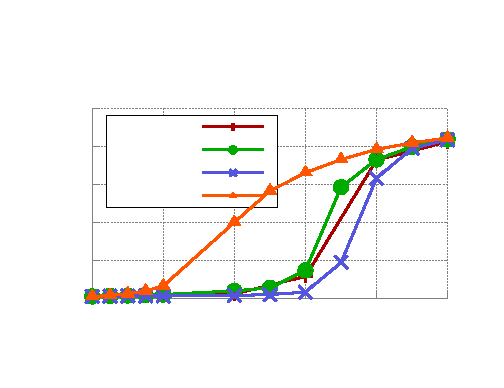
\includegraphics{latex_plots/modelB_to_modelA0_3_all}}%
    \gplfronttext
  \end{picture}%
\endgroup
=======
>>>>>>> d0c993ed222f71e795df2da0bffd16f549b80e42
